\documentclass[a4paper,10pt]{article}

\usepackage{graphicx}
\usepackage{float}

\title{LaTex test in VS Code}
\author{Océane Patiny}
\date{\today}

\begin{document}

\maketitle

\section*{Introduction}

The paragraph tha follows is a quote from a 2000 years old text on which Lorem Ipsum is based.
Sed ut perspiciatis unde omnis iste natus error sit voluptatem accusantium doloremque laudantium, totam rem aperiam, eaque ipsa quae ab illo inventore veritatis et quasi architecto beatae vitae dicta sunt explicabo. Nemo enim ipsam voluptatem quia voluptas sit aspernatur aut odit aut fugit, sed quia consequuntur magni dolores eos qui ratione voluptatem sequi nesciunt. Neque porro quisquam est, qui dolorem ipsum quia dolor sit amet, consectetur, adipisci velit, sed quia non numquam eius modi tempora incidunt ut labore et dolore magnam aliquam quaerat voluptatem. Ut enim ad minima veniam, quis nostrum exercitationem ullam corporis suscipit laboriosam, nisi ut aliquid ex ea commodi consequatur? Quis autem vel eum iure reprehenderit qui in ea voluptate velit esse quam nihil molestiae consequatur, vel illum qui dolorem eum fugiat quo voluptas nulla pariatur?\\

This seems to be a pretty practical thingy.\\

Let's add an image, or no, a formula first.

\begin{equation}
    \Delta = \sqrt{b^2 - 4ac}
\end{equation}

Ok so now this worked and I would like to add a pretty image of a cat.


\begin{figure}[H]
    \centering
    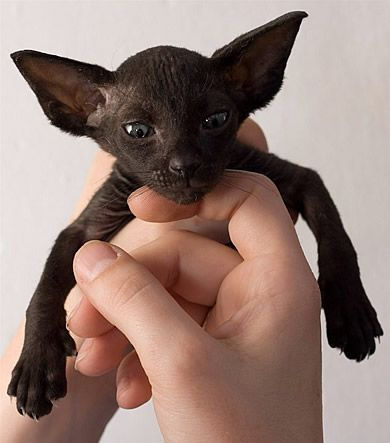
\includegraphics[width = 0.4\textwidth]{sphinx.jpg}
    \caption{Cät (photoscats.com).}
    \label{fig:scheme1}
\end{figure}



\label{Lastpage}
\end{document}


